\documentclass{article}
\usepackage[utf8]{inputenc}
\usepackage{amsmath,amsthm,amsfonts,amssymb,amscd}
\usepackage[a4paper,hmargin=0.8in,bottom=1.3in]{geometry}
\usepackage{lastpage,enumerate,fancyhdr,mathrsfs,xcolor,graphicx,listings,hyperref,enumitem}
\author{Hardik Rajpal}
\title{Notes from \href{https://zerodha.com/varsity/chapter/what-to-expect/}{Trading Systems}}
\hbadness 100001
\begin{document}
\maketitle
\section{What To Expect}
Trading techniques, not trading systems, are of the sort:
\begin{itemize}
    \item System-Deduction-based trading
    \item Trade because your gut says so
    \item Trade because my friend says so
    \item Trade because the guy on TV says so
    \item Trade because my broker says so
\end{itemize}
A trading system (1) takes some inputs from the market, (2) runs specific logic, implemented
by you and (3) gives you an output. The onus of deciding whether or not to make
the trade is still on the human trader.\\
The module plans to discuss:
\begin{enumerate}
    \item Pair trading (not related to that thing you suggested to your wife!)
    \item Volatility based Delta hedging
    \item Calendar spreads
    \item Momentum strategy (Portfolio approach)
\end{enumerate}
No trading system is complete without backtesting, which is not covered by this module.
\section{Pair Trading Logic}
If two entities A and B (listed on the stock market) are related (have similar business landscapes and environments), their stock prices are expected to behave similarly (barring any anomalies). If we observe that SP(A) moves up by X\% on a particular day, we expected SP(B) to move up by y\% too. If at the moment, this expected change has not occurred, we say that B has the cheaper stock and A has expensive stock.\\
\textbf{Cheaper Stock:} The upward change in its price is less than that of the stock prices of entities similar to it. It is undervalued.\\
\textbf{Expensive Stock:} The upward change in its price is more than that of stock prices of entities similar to it. It is overvalued.\\
\textbf{Anomaly: }An event that triggers the changes in stock prices of two closely related entities to deviate. Anomalies in stock prices give us an opportunity to trade.\\
The bulk of pair trading revolves around:
\begin{enumerate}
    \item Identifying the relationship between two \emph{pair} stocks.
    \item Quantifying their relationship.
    \item Tracking the behaviour of this relationship on a daily basis.
    \item Looking for anomalies in the price behaviour.
\end{enumerate}
Two popular techniques to define the relationship between two stocks are based on
\textbf{price spreads and ratios} and \textbf{linear regression}.\\
Note that pair trading is not a market neutral strategy, because although you may
be long and short, you are long and short on two different stocks. To be market 
neutral, you need to long and short on the same stock at the same time.
In the ``calendar spread'',youare long and short on the same stock, expiring on
two different dates.\\
Pair trading can also be called `Relative Value Trading', as we are trying
to profit from the relative value of the two securities. It's also called 
`Statisical Arbitrage'. (Arbitrage refers to the simultaneous buying and selling
of commodities to benefit from the difference in their prices.)\\
Note that undervalued and overvalued are relative terms. How this
relative value is calculated is discussed next.
\section{Pair Trading Method 1: Correlation}
\subsection{Tracking Pairs}
Here comes some jargon:
\begin{itemize}
    \item \textbf{Stock Value: }What someone is willing to pay for it; what the stock is worth.
    \item \textbf{Stock Price: }The stock's current value to buyers and sellers.
    \item \textbf{Spreads:} The word refers to the difference between the closing values of two stocks (in the pair trading world).\\
    \begin{center}
        spread = CV(A) - CV(B)
    \end{center}
    Historical spread refers to spread data collected on a daily basis.
    \item \textbf{Differential:} It refers to the difference in closing prices of two stocks.
    \begin{center}
        differential = CP(A) - CP(B)
    \end{center}  
    Differentials are not great to track pairs on an intraday basis; they're best used as an end-of-day basis. Spreads can be used to track pairs on an intraday basis.
    \item \textbf{Ratio:} It's the stock price of A by the stock price of B.
    \begin{center}
        ratio = SP(A)/SP(B)
    \end{center}
    \item \textbf{Divergence: }If the ratio or spread between two stocks is expected to move apart (the graph moves up), we call it divergence. Then, we try to make money by setting up a divergence trade.
    \item \textbf{Convergence: }If the ratio of spread is expected to decrease (the graph goes down), we call it convergence. We try setting up a convergence trade.
\end{itemize}
The question to make money then is, of course, is the pair going to diverge or converge? Even before this, how do we qualify two stocks as a pair? The second 
question's answer is correlation. The sign of the correlation tells us how the direction of changes are related and the magnitude tells us how strongly.
Note that correlation allows for drawing probabilistic conclusions.\\
The correlation data only makes sense if the data is stationary around the mean; 
the dataset sticks close to the average values.\\
\fbox{Not clear about the difference between spread and differential.}
\subsection{Pair Stats}
\subsubsection{Correlation and its Types}
To estimate the correlation between the stock prices of two entities, say A and B,
ensure that you have the same number of data points for both A and B (and at the
same points in time). Also, the data should be ``cleaned'' for corporate actions such as bonus, splits, etc. We estimate daily returns for both stocks:
\begin{center}
    daily return at day t = (CP(t)/CP(t-1)) - 1
\end{center}
\begin{center}
    absolute per day change = CP(t) - CP(t-1)
\end{center}
We can use the \texttt{=Correl(col1, col2)} function in excel suitably. Note that
the correlation function is commutative. the correlation calculated on the closing prices of stocks is called ``closed correlation.''
\subsubsection{Statistic Variables}
\textbf{Mean:} The arithmetic average. $\overline{x} = \sum_{i\in [n]}{x_i}/n$\\
\textbf{Median:} The middle number if n is odd ($x_{(n+1)/2}$), else it's $\frac{x_{n/2}+x_{(n/2) + 1}}{2}$.\\
\textbf{Mode:} The most frequently occuring value: $x_M = \text{argmax}_{x_i}{freq(x_i)}$
\subsection{Pre Trade Setup}
\subsubsection{Normal Distro}
Note that the variables spread, differential and ratio are expected to be 
normally distributed. Here are some normal distribution facts (100/100):
\begin{itemize}
    \item Within the 1st standard deviation lies 68\% of the data.
    \item Within the 2nd standard deviation lies 95\% of the data.
    \item Within the 3rd standard deviation lies 99.7\% of the data.
\end{itemize}
\subsubsection{Descriptive Stats}
Excel functions \texttt{average(), median(), mode.mult()} are useful in the 
pursuit of mean, median and mode. Standard deviation is the most common measure 
variability and is used to determine the volatility of stock markets or other 
investments. (Excel: \texttt{Stdev.p()})
\begin{equation}
    \sigma = \sqrt{\sum_{i\in [n]}{(x_i-\overline{x})^2}}
\end{equation}
Absolute deviation is also known as mean absolute deviation (MAD).
\begin{equation}
    MAD = \sum_{i\in[n]}{|x_i - \overline{x}|}
\end{equation}
MAD is seldom preferred because of the complications brought along with the
absolute value. (Excel: \texttt{avedev()})\\
The mean, median, mode, standard deviation and absolute deviation are 
collectively known as \textbf{the basic descriptive statistics}.
\subsubsection{The Standard Deviation Table}
\begin{center}
    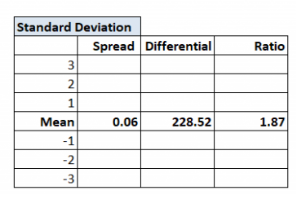
\includegraphics{rsrc/stdtable.png}
\end{center}
We use the normal distribution as a basis to deduce probabilistic conclusions like:
\begin{itemize}
    \item If the current data point are at a far end of the bell shape, say ~$3\sigma$, the next data point is likely to be closer to the mean with probability 99.7\%. We say with 99.7\% confidence that there is only 0.3\% chance for the point to be further away from the mean.
    \item On second thoughts, shouldn't the probability of return be 99.7 + 0.15
    = 99.85\% and the probability of it going higher be 0.3/2 = 0.15\%?
\end{itemize}
\subsection{The Density Curve}
\subsubsection{Selecting the Variable}
We need to pick one of spread, differential and ratio to avoid getting confused
by conflicting signals. It's up to the trader to choose the variable they are 
most comforable with. We go ahead with the ratio in the discussions ahead.
\subsubsection{The Trade Trigger}
Wherever the selected variable (ratio) is today, there is a great chance
(quantifiable) that it will return to the running mean over the next few days.
This phenomenon is known in the hood as \textbf{mean reversion} or \textbf{reversion to mean}. Think of the ratio as an abstract form of stock:
 we say that we can ``short'' (sell) the ratio when it's
significantly above the mean (only to buy it back when it returns to the mean,
hence profiting) or ``long'' (buy) it when it is significantly below 
the mean (only to sell it back when it returns, hence profiting).\\
\textbf{Key Trigger to Trade:} The ratio's current value w.r.t. its mean.\\
\indent \textbf{Above the mean} $\implies$ short the ratio!\\
\indent \textbf{Below the mean} $\implies$ long the ratio!\\
The only question that remains is:
\begin{center}
    \fbox{How far away from the mean do we wait for the ratio to go before acting?}
\end{center}
\subsubsection{The Density Curve}
We need to initiate a trade only when we are reasonably ceratin that the
ratio will slide down to the mean value, \textbf{as quickly as possible.}. Here
we put our faith in the good ol' Normal Distribution's properties. If the ratio
is 3 SDs away from the mean, the chance of it going further away is 0.3\%; the ``chance of it reverting to the mean'' is 99.7\%. Using this idea, we filter
out opportunities to initiate trades only at points where the likelihood of mean
reversion is high.\\
As the trigger to trade depnds on the ratio and its standard deviation, we need to track the daily standard deviation of the ratio as opposed to the ratio itself.
This is achieved by tracking the `Density Curve' of the ratio.\\
The density curve is the continous counterpart of the relative frequency
histogram; the bin sizes tend to zero. This is the cumulative distribution function, cdf(x). In Excel, the function NORM.DIST function is useful for this:\\
NORM.DIST(x, $\mu$, $\sigma$, isCumulative)\\
if(isCumulative):\\
\indent NORM.DIST(x, $\mu$, $\sigma$, isCumulative) $\equiv$ cdf(x;$\mu$, $\sigma$)\\
else:\\
\indent NORM.DIST(x, $\mu$, $\sigma$, isCumulative) $\equiv$ pdf(x;$\mu$, $\sigma$)
\subsection{The Pair Trade}
Here are some density curve (cdf(x)) facts (100/100):
\begin{itemize}
    \item cdf($x_{curr}$) = 0.997 $\implies$ $x_{curr} = \mu+3\sigma$
    \item cdf($x_{curr}$) = 0.974 $\implies$ $x_{curr} = \mu+2\sigma$
    \item cdf($x_{curr}$) = 0.84 $\implies$ $x_{curr} = \mu+\sigma$
    \item cdf($x_{curr}$) = 0.16 $\implies$ $x_{curr} = \mu-\sigma$
    \item cdf($x_{curr}$) = 0.025 $\implies$ $x_{curr} = \mu-2\sigma$
    \item cdf($x_{curr}$) = 0.003 $\implies$ $x_{curr} = \mu-3\sigma$
\end{itemize}
General thresholds for trading short and long are given below. The target
value of the density curve is the value you want the density curve to go to
after you make the trade for considerable profit.
\begin{itemize}
    \item cdf($x_{curr}$) $\in$ (0.003,0.025) $\implies$ long.
    (Stoploss=0.003 or higher, target = 0.25 or lower)
    \item cdf($x_{curr}$) $\in$ (0.975,0.997) $\implies$ short.
    (Stoploss=0.997 or higher, target = 0.975 or lower)
\end{itemize}
In concrete terms, if the ratio is Stock A/Stock B,
\begin{itemize}
    \item long trade $\implies$ buy Stock A and sell Stock B.
    \item short trade $\implies$ sell Stock A and buy Stock B.
\end{itemize}
Remember it as the numerator being the dominating term and long (buy) $\implies$
buy the numerator while short (sell) $\implies$ sell the numerator. The
denominator always suffers the alternative fate.
\subsubsection{Real Talk}
\begin{itemize}
    \item For a given pair, one can expect at most 2-3 signals in a year; we need to observe multiple pairs to continuously find profit opportunities.
    \item We have not discussed neutrality of both the positions, which is apparently a key angle.
    \item As pair trading is a margin money guzzler, one needs to have sufficient funds to pair trade.
\end{itemize}
\section{Pair Trading Method 2: Statistical Arbitrage}
This is also known as \textbf{Relative Value Trading}.
\subsection{Straight Line Equation}
Straigh line equation: $y = mx + \epsilon$
\subsection{Linear Regression}
Given $\{x_i,y_i\}_{i\in[n]}$, we estimate $m$ and $\epsilon$.\\
\begin{center}
    residual = $y_i - (mx_i + \epsilon)$
\end{center}
\subsection{The Error Ratio}

\end{document}